\documentclass[12pt,a4paper]{article}
\usepackage[utf8x]{inputenc}
\usepackage{ucs}
\usepackage[spanish]{babel}
\usepackage{amsmath}
\usepackage{amsfonts}
\usepackage{amssymb}
\usepackage{makeidx}
\usepackage{graphicx}
\usepackage[hidelinks]{hyperref}
\usepackage[left=2cm,right=2cm,top=2cm,bottom=2cm]{geometry}
\author{Reyes Alvarez Ulises Isaac\\4.B  Ing. Mecatrónica\\Mtro. Carlos Enrique Morán Grabito\\ Sistemas electrónicos de Interfaz}
\title{Amplificadores Clase B}
\begin{document}
\maketitle
\begin{figure}[hbtp]
\centering

\includegraphics[scale=1.7]{Pictures/Universidad.png}
\end{figure}

\newpage
\section*{Amplificadores Clase B}
\section{Características}
Los amplificadores de clase B se caracterizan por tener intensidad casi nula a través de sus transistores cuando no hay señal en la entrada del circuito, por lo que en reposo el consumo es casi nulo. Se les denomina amplificador clase B, cuando el voltaje de polarización y la máxima amplitud de la señal entrante poseen valores que hacen que la corriente de salida circule durante el semiciclo de la señal de entrada.\\
La característica principal de este tipo de amplificadores es el alto factor de amplificación.
Amplificadores clase AB: Estos básicamente son la mezcla de los dos anteriores. Cuando el voltaje de polarización y la máxima amplitud de la señal entrante poseen valores que hacen que la corriente de salida circule durante menos del ciclo completo y más de la mitad del ciclo de la señal de entrada, se les denomina: Amplificadores de potencia clase AB.\\
Dado que ocupa un lugar intermedio entre los de clase A y AB, cuando el voltaje de la señal es moderado funciona como uno de clase A, cuando la señal es fuerte se desempeña como uno de clase B, con una eficiencia y deformación moderadas.\\
\begin{figure}[hbtp]
\centering
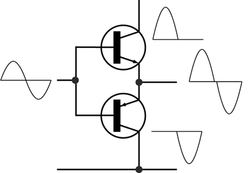
\includegraphics[scale=0.6]{Pictures/ClaseB.png}
\caption{Amplificador Clase B}
\end{figure}

Los amplificadores de Clase B usan dos o más transistores polarizados de tal forma que cada transistor solo conduce durante un medio ciclo de la onda de entrada.\\
Para mejorar la eficiencia de potencia total del amplificador de clase A previo reduciendo la potencia desperdiciada en forma de calor, es posible diseñar el circuito amplificador de potencia con dos transistores en su etapa de salida produciendo lo que comúnmente se denomina amplificador de clase B también. conocido como una configuración de amplificador push-pull.\\
\begin{figure}[hbtp]
\centering
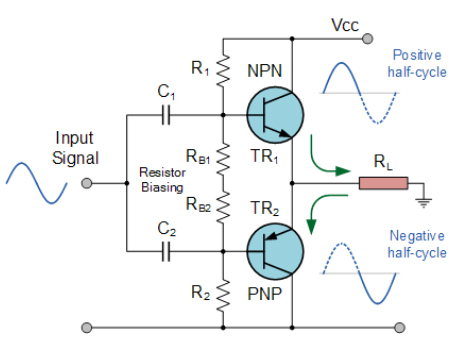
\includegraphics[scale=0.35]{Pictures/0.jpg}
\caption{Amplificadores Push-Pull}
\end{figure}


\newpage
\section{Funcionamiento}
Un amplificador de potencia funciona en clase B cuando la polarización de dc deja al transistor casi apagado de manera que el transistor se enciende cuando a este se le aplica una señal en ac. Es decir que le transistor conducirá corriente solamente para una mitad de ciclo de la señal.\\
Ahora para obtener una señal de ciclo completo será necesario utilizar dos transistores y lograr que cada uno de ellos conduzca durante medios ciclos opuestos, y al tener esta operación combinada se obtiene un ciclo completo de señal de salida.\\
Dado que una parte del circuito "empuja" a la señal de arriba durante una mitad del ciclo y la otra parte "jala" la señal hacia abajo durante la otra mitad del ciclo, el circuito por ende se denomina de contrafase circuito push-pull.
\begin{figure}[hbtp]
\centering
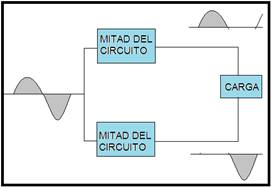
\includegraphics[scale=1.2]{Pictures/1.jpg}
\caption{Representación en bloques de la operación en contrafase}
\end{figure}

Los transistores de potencia empleados en el circuito de contrafase son capaces de entregar la potencia deseada a la carga, y la operación clase B de estos transistores proporciona una diferencia mayor que la que era posible mediante un solo transistor en la operación clase A.
\begin{figure}[hbtp]
\centering
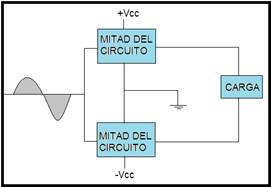
\includegraphics[scale=1.2]{Pictures/2.jpg}
\caption{Conexión del amplificador en contrafase con la carga mediante dos fuentes de voltaje}
\end{figure}

\newpage
\section{Circuito Amplificador de Transformador Push-pull de Clase B}
El circuito anterior muestra un circuito amplificador Clase B estándar que utiliza un transformador de entrada con toma central compensada, que divide la señal de forma de onda entrante en dos mitades iguales y que están desfasadas 180° entre sí. Otro transformador con toma central en la salida se utiliza para recombinar las dos señales que proporcionan la mayor potencia a la carga. Los transistores utilizados para este tipo de circuito amplificador push-pull de transformador son ambos transistores NPN con sus terminales de emisor conectados entre sí.
Aquí, la corriente de carga se comparte entre los dos dispositivos de transistor de potencia a medida que disminuye en un dispositivo y aumenta en el otro a lo largo del ciclo de señal, reduciendo el voltaje y la corriente de salida a cero. El resultado es que ambas mitades de la forma de onda de salida ahora oscilan desde cero hasta el doble de la corriente de reposo, reduciendo así la disipación. Esto tiene el efecto de casi duplicar la eficiencia del amplificador a alrededor del 70 por ciento.\\
El funcionamiento del amplificador de clase B tiene polarización CC cero ya que los transistores están polarizados en el corte, por lo que cada transistor solo conduce cuando la señal de entrada es mayor que la tensión del emisor base . Por lo tanto, en la entrada cero hay salida cero y no se consume energía.\\
\begin{figure}[hbtp]
\centering
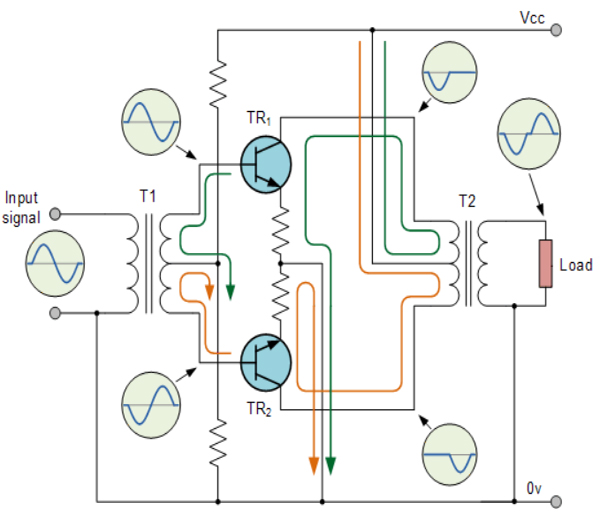
\includegraphics[scale=0.5]{Pictures/3.jpg}
\caption{Amplificador de Transformador Push - Pull}
\end{figure}

\newpage
\subsection{Curvas de características de salida de clase B}
El amplificador de clase B tiene la gran ventaja sobre sus primos de amplificador de clase A en que ninguna corriente fluye a través de los transistores cuando están en estado de reposo (es decir, sin señal de entrada), por lo tanto no se disipa potencia en los transistores de salida o transformador cuando no hay señal presente a diferencia de las etapas de amplificador de Clase A que requieren un sesgo de base significativo, disipando así gran cantidad de calor, incluso sin presencia de señal de entrada.\\

Por lo tanto, la eficiencia total de conversión del amplificador es mayor que la de la Clase A equivalente, alcanzando eficiencias tan altas como 70 por ciento, lo que resulta en casi todos los tipos modernos de amplificadores push-pull operados en este modo Clase B.\\
\begin{figure}[hbtp]
\centering
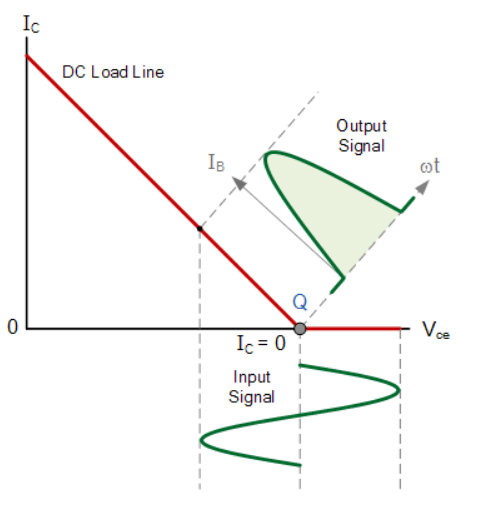
\includegraphics[scale=0.5]{Pictures/4.jpg}
\caption{Curvas del Amplificador de Transformador Push - Pull}
\end{figure}

\newpage
\section{Rendimiento del circuito}
El Amplificador de Potencia en simetría complementaria presenta un excelente rendimiento, pues si señal de entrada el circuito absorbe una corriente mínima y, cuando ésta está en presente, la mayor parte de la potencia consumida es transferida a la carga.\\\\
La potencia absorbida de la fuente vendrá determinada por la corriente media en la carga y la tensión de alimentación Vcc (despreciando nuevamente la corriente absorbida por el divisor de polarización de bases R1, P y R2), así: 
\begin{equation}
Pcc = \ Irl \cdot Vcc=\frac{Vceq}{\pi \cdot Rl} \cdot Vcc=\frac{Vcc}{2 \pi \cdot Rl} \cdot Vcc=\frac{Vcc^{2}}{2 \pi \cdot Rl}
\end{equation}
donde Irl es la intensidad media absorbida por la carga.\\

La máxima potencia disipada por la carga presentará cuando la señal de entrada sea máxima y el punto de trabajo recorra toda la recta de la carga, entonces: 
\begin{equation}
Vrlpp max = Vcc
\end{equation}
y
\begin{equation}
Pl max = Vcc^{2} 
\end{equation}
donde
\begin{equation}
n = \frac{Pl max}{Pcc} \cdot 100 = \frac{Vcc^{2} \cdot 2 \pi \cdot Rl}{8Rl \cdot Vcc ^{2}} \cdot 100 
\end{equation}

\section{Ventajas}
* Posee bajo consumo en reposo.\\
* Aprovecha al máximo la Corriente entregada por la fuente.\\
* Intensidad casi nula cuando está en reposo.\\

\section{Desventajas}
* Producen armónicos, y es mayor cuando no tienen los transistores de salida con las mismas características técnicas, debido a esto se les suele polarizar de forma que se les introduce una pequeña polarización directa. Con esto se consigue desplazar las curvas y se disminuye dicha distorsión.

\section{Aplicaciones}
* Sistemas telefónicos.\\
* Transmisores de seguridad portátiles.\\
* Sistemas de aviso, aunque no en audio.\\

\section*{Referencias bibliográficas}
\url{https://www.ecured.cu/Amplificador_Clase_B}\\
\url{https://www.monografias.com/trabajos89/amplificador-potencia-clase-b/amplificador-potencia-clase-b.shtml}\\
\url{http://tutorialesdeelectronicabasica.blogspot.com/2018/06/amplificador-de-clase-b-y-amplificador.html}\\
\url{https://electronicavm.files.wordpress.com/2011/03/amplificadores-clase-a-y-b1.pdf}\\

\end{document}